\documentclass[10pt,a4paper]{article}
\usepackage[latin1]{inputenc}
\usepackage{amsmath}
\usepackage{amsfonts}
\usepackage{amssymb}
\usepackage{graphicx}
\bibliography{FEM_ref}
%\usepackage{biblatex}
\title{Finite Element Method Computer Assignment 4.1.1}
\begin{document}

\begin{figure}[t]
	\centering
	
\includegraphics[width=0.5\textwidth]{TU_d_line_P1_color_1.jpg}
\end{figure}

\begin{center}
	\textbf{Computer Assignment 4.1.1}\\
	\textbf{MMP Finite Element Methods (WI4243AP-FE)}
	\begin{tabular}{lr}
		\textbf{Shaikh Bechan} & \textbf{4146425}\\
		\textbf{Zubin Ramlakhan} & \\
	\end{tabular}
\end{center}

\section{Introduction}
The following is a report containing the evaluation of the heat equation with the finite element method.
To solve the two-dimensional heat equation numerically, the finite element method is applied. To that end the minimization problem corresponding to the partial differential in question is derived. The solution of the minimization problem is approximated with the finite element method by deriving the element stiffness matrix and element stiffness vector using triangular and line elements.

\section{The Heat Equation}
	\begin{figure}[h]
		\centering
		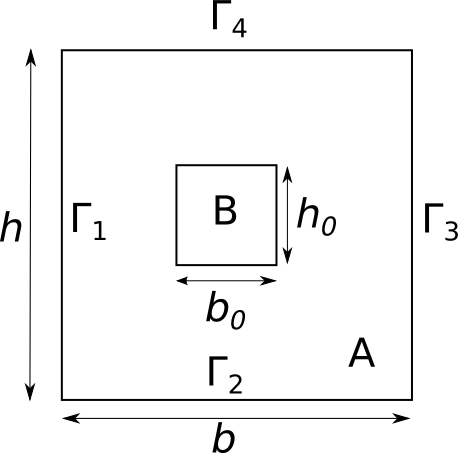
\includegraphics[width=0.6\textwidth]{schem.png}
		\caption{Rectangular plate made of two materials, $A$ and $B$.}
		\label{fig:schem}
	\end{figure}
Consider the rectangular plate shown in figure \ref{fig:schem}, with width, $b$, and height, $h$. In the center of the plate is a rectangular part, of a different material, with width, $b_0$ and height, $h_0$. $A$ denotes the outer part of the plate while $B$ denotes the inner part.

The situation is stationary and the effects of convection and sources are absent. Thus the heat equation is simply defined by the conduction (diffusion) term as shown in \eqref{eq:heat}

\begin{equation}\label{eq:heat}
	-\nabla \cdot (k \nabla T) = 0
\end{equation}

with heat conductivity $k$ and temperature $T$. The thermal conductivity is different in each material, i.e. $ k|_A = k_A $ and $k|_B = k_B $.\\

The boundary of $A$, $\partial A$,  is divided in four segments such that $\partial A = \Gamma_1 \cup  \Gamma_2 \cup  \Gamma_3 \cup  \Gamma_4$. On these boundaries the following conditions hold:

\begin{align}
T\rvert_{\Gamma_1\cup\Gamma_3}& = T_0 \label{eq:bc13}\\
\nabla T\rvert_{\Gamma_2} &= 0\label{eq:bc2}\\
k\frac{\partial T}{\partial n}\rvert_{\Gamma_4}=&-\alpha(T_w - T_{\infty})\label{eq:bc4}
\end{align}

In words, the temperature at boundaries $\Gamma_1$ and $\Gamma_3$ are held constant at $T=T_0$. The flux at $\Gamma_2$ is zero. $\Gamma_4$ obeys Newton's heat transfer relation with the environment temperature $T_{\infty}$ and the temperature at the wall $T_w$.\\

In this problem a symmetry plane is present. This plane runs along the midsection of the plate in the vertical direction. Here, to ensure symmetry, the gradient of the temperature must be zero.

\section{Minimization problem}
A partial differential equation can be related to an equivalent minimization problem with the following theorem\cite{Kan2008}:\\

\textit{Let $L$ be a linear, symmetric, positive differential operator defined of space $\Sigma$ and let}
\begin{equation}\label{eq:pde}
Lu=f
\end{equation}
\textit{Then the solution $u$ minimizes the functional}
\begin{equation}\label{eq:min}
I(u) = \underset{\Omega}{\int}\{\frac{1}{2}uLu-uf\}d\Omega
\end{equation}  \textit{over the space $\Sigma$. On the other hand, if $u$ minimizes \eqref{eq:min} then $u$ satisfies \eqref{eq:pde}} \\

Another requirement $u$ should obey is homogeneous boundary conditions, a requirement $T$ fails. Even so, this theorem can still be utilized by adapting it or by making the boundary conditions homogeneous. The latter is simpler to accomplish.

Let $Lu=f$ with non-homogeneous boundary equations and suppose that there is another smooth function $w$ that also satisfies the same non-homogeneous boundary conditions. Now let 
\begin{equation}\label{eq:v}
v=T-w
\end{equation}
$T$ and $w$ satisfy the same non-homogeneous boundary conditions, therefore $v$ satisfies homogeneous boundary conditions. Now the theorem can be applied to $v$ as it meets all the requirements. \\

\begin{equation}\label{rhsv}
Lv=LT-Lw=f-Lw
\end{equation}
so the corresponding minimization problem is given by 

\begin{equation}\label{eq:min1}
\underset{v\in\Sigma} {min}I(v) = \frac{1}{2}\underset{\Omega}{\int}vLvd\Omega-\underset{\Omega}{\int}v(f-Lw)d\Omega
\end{equation}

Substituting \eqref{eq:v} into \eqref{eq:min1} yields

\begin{equation}\label{eq:min2}
\underset{v\in\Sigma} {min}I(v) = \frac{1}{2}\underset{\Omega}{\int}(T-w)L(T-w)d\Omega-\underset{\Omega}{\int}(T-w)(f-Lw)d\Omega
\end{equation}

$f=0$ and $L = -\nabla\cdot( k\nabla)$ according to \eqref{eq:heat}, so \eqref{eq:min2} is rewritten as

\begin{equation}\label{eq:min3}
	\begin{split}
	\underset{v\in\Sigma} {min}I(v) & = -\frac{1}{2}\underset{\Omega}{\int}(T-w)\nabla\cdot(k\nabla(T+w))d\Omega\\
	&=\frac{1}{2}\underset{\Omega}{\int}\nabla (T-w)(k\nabla(T+w))-\nabla\cdot\{(T-w)(k\nabla(T+w))\}d\Omega\\
	&=\frac{1}{2}\underset{\Omega}{\int}\nabla (T-w)(k\nabla(T+w))d\Omega - \frac{1}{2}\underset{\Gamma}{\int}(T-w)(k\nabla(T+w))\cdot\textbf{\^{n}} d\Gamma\\
	&=\frac{1}{2}\underset{\Omega}{\int}\nabla T\cdot k \nabla T d\Omega - \frac{1}{2}\underset{\Omega}{\int}\nabla w\cdot k \nabla w d\Omega\\  &-\frac{1}{2}\underset{\Gamma}{\int}(T-w)(k\nabla(T+w))\cdot\textbf{\^{n}} d\Gamma
	\end{split}
\end{equation}
where the product rule and subsequent Gauss theorem is applied to expand the integral in two volume integrals and one boundary integral. The second integral is independent on $T$ and thus has no influence on the minimization and can be neglected. \\

The boundary integral is evaluated over four boundaries by taking in account the boundary conditions \eqref{eq:bc13}$-$\eqref{eq:bc4}. 

\begin{align}\label{eq:bcint13}
	\frac{1}{2}\underset{\Gamma_1\cup\Gamma_3}{\int}(T_0-T_0)(k\nabla(T+w))\cdot\textbf{\^{n}} d\Gamma &= 0\\
	\frac{1}{2}\underset{\Gamma_2}{\int}(T-w)(k(0+0))\cdot\textbf{\^{n}} d\Gamma & = 0\label{eq:bcint2}\\ 
	\frac{1}{2}\underset{\Gamma_4}{\int}(T-w)(k\nabla(T+w))\cdot\textbf{\^{n}} d\Gamma & = \frac{1}{2}\underset{\Gamma_4}{\int}Tk\frac{\partial T}{\partial n}d\Gamma - \frac{1}{2}\underset{\Gamma_4}{\int}wk\frac{\partial w}{\partial n}d\Gamma\nonumber\\
	&=-\frac{1}{2}\underset{\Gamma_4}{\int}\alpha T(T_w-T_{\infty})d\Gamma \label{eq:bcint4}
\end{align}
where $\frac{1}{2}\underset{\Gamma_4}{\int}wk\frac{\partial w}{\partial n}d\Gamma$ is neglected as it too is independent of $T$.

Finally, the minimization problem is given by
\begin{equation}\label{eq:minf}
\underset{T\in\Sigma} {min}I(v) =\frac{1}{2}\underset{\Omega}{\int}k\lvert\nabla T \rvert ^{2}  d\Omega + \frac{1}{2}\underset{\Gamma_4}{\int}\alpha T(T_w-T_{\infty})d\Gamma 
\end{equation}
with $\Sigma: \{T\rvert\quad T\rvert_{\Gamma_1\cup\Gamma_3}=T_0\rvert\quad \nabla T\rvert_{\Gamma_2}=0\}$. The boundary conditions \eqref{eq:bc13} and \eqref{eq:bc2} are essential boundary conditions.
\section{References}

\end{document}
